%                                                                 aa.dem
% AA vers. 9.1, LaTeX class for Astronomy & Astrophysics
% demonstration file
%                                                       (c) EDP Sciences
%-----------------------------------------------------------------------
%
% \documentclass[referee]{aa} % for a referee version
%\documentclass[onecolumn]{aa} % for a paper on 1 column  
%\documentclass[longauth]{aa} % for the long lists of affiliations 
%\documentclass[letter]{aa} % for the letters 
%\documentclass[bibyear]{aa} % if the references are not structured 
%                              according to the author-year natbib style

%

\documentclass{aa}  

%
\usepackage{graphicx}
\usepackage{amsmath,amsfonts,amssymb}
\usepackage{natbib}


%%%%%%%%%%%%%%%%%%%%%%%%%%%%%%%%%%%%%%%%
\usepackage{txfonts}
\usepackage{xcolor}

\usepackage{blindtext}
%%%%%%%%%%%%%%%%%%%%%%%%%%%%%%%%%%%%%%%%
% \usepackage[options]{hyperref}
% To add links in your PDF file, use the package "hyperref"
% with options according to your LaTeX or PDFLaTeX drivers.
\usepackage{float}
%\usepackage{stfloats}
\usepackage{dblfloatfix}
\usepackage{afterpage}
\usepackage{ifthen}
\usepackage[morefloats=12]{morefloats}

\usepackage{placeins}
\usepackage{multicol}
%\usepackage[breaklinks,colorlinks,citecolor=blue]{hyperref}
\bibpunct{(}{)}{;}{a}{}{,}
\usepackage[switch]{lineno}
\definecolor{linkcolor}{rgb}{0.6,0,0}
\definecolor{citecolor}{rgb}{0,0,0.75}
\definecolor{urlcolor}{rgb}{0.12,0.46,0.7}
\usepackage[breaklinks, colorlinks, urlcolor=urlcolor,
    linkcolor=linkcolor,citecolor=citecolor,pdfencoding=auto]{hyperref}
\hypersetup{linktocpage}
\usepackage{bold-extra}

%Planck style file, to be used with A&A style to produce Planck papers for publication.
%
% version 28 September 2010 --- useful macros --- CRL
% version 17 October 2010   --- first cut at important instrument values, from Daniele Mennella and
%                               Francois Bouchet, 13 October 2010 --- CRL
% version 18 October 2010   --- LFI FWHM changed to one value per feed, rather than M & S separately
%                               LFI FWHM uncertainties added for individual feeds.  Corrections made
%                               to LFI values. --- Andrea Zacchei
% version 24 October 2010   --- added to and corrected definitions.  No changes made to instrument
%                               quantities. --- CRL 
% version 31 October 2010   --- added definition of \muKHz. --- CRL
%
% version 15 November 2010  --- fixed conflict with aa.cls in definition of \endtable
%                               by naming the command below "\endPlancktable".  See section
%                               13.16 of the Style Guide.
%
% version 06 December 2010  --- Set up names with and without units.
%                               Add \allearlypapers command to ensure that all early papers are
%                               included in the reference list.
%                               Define macro for the name of the 4He JT cooler.
%
% version 07 December 2010  --- removed extraneous "planck2011-1.2" entry in \allearlypapers
%
% version 12 December 2010  --- added \endPlancktablewide command to set tablenotes to the full
%                               page width in the \begin{table*}...\end{table*} environment when
%                               the ``twocolumn'' option is specified in the \documentclass command.
%                               (It would be more elegant to extract the appropriate width from the
%                               aa.cls system at the time of execution, but that is buried more
%                               deeply in the system than I investigated.)
%
% version 05 January 2011   --- added unit \MJysr.  HFI performance values updated per FRB email
%                               01/05/2011 02:38-0800, and Brendan Crill email 01/05/2011 18:08 -0800.
%
% version 06 January 2011   --- changed \scriptscriptstyle primes to \scriptstyle, to better match the
%                               tx fonts used by A&A.
%
% version 07 January 2011   --- modified \allearlypapers to correspond with final early paper list.  
%                               Fixed 545 GHz center frequency.
%
% version 07 January 2011b  --- changed LFI white-noise sensitivity numbers to correct problem with units
%
% version 05 July 2011      --- added \Msol and \Lsol to get the symbols for solar mass and luminosity.
%                               Deleted previous definitions of \solar and \sol, which were equivalent
%                               to the new \Msol.
%
% version 16 August 2011    --- changed comments on \endPlancktable and \endPlancktablewide for clarity
%
% version 11 September 2011 --- changed definition of \tablenote to make footnote labels italic, as per A\&A
%
% version 26 April 2011     --- changed definition of \Planck to agree with what is said in the Style Guide (!)
%
% version 04 Dec 2013       --- included 2013 results references
%
% version 17 Jan 2014       --- included fix to bibtex file v4.3, i.e. \providecommand{\sorthelp}[1]{}
%
% version 26 Jul 2014       --- fixed incompatibility problem with aa.cls v8.0 and v8.2.  v8.2 should now be used
%                               for all Planck papers.
%                           --- fixed problem in definition of "\all2013resultspapers" that introduced a blanck
%                               into the reference to p06b.
%                           --- removed all the parameter definition stuff at the end.  We weren't using it, and
%                               it took up a lot of space.
%
% version 28 Jan 2015       --- added "\alltwentyfiftennresultspapers" and corrected "\all2013resultspapers" to
%                               "\all20thirteenresultspapers",
%
% Usage:  after the \documentclass[traditabstract]{aa} command in the La\TeX\ input file,
%         add this command:      \input Planck.tex


\def\setsymbol#1#2{\expandafter\def\csname #1\endcsname{#2}}
\def\getsymbol#1{\csname #1\endcsname}

%-----------------------------------------------------------------------
% Planck
%-----------------------------------------------------------------------
\def\Planck{\textit{Planck}}

%-----------------------------------------------------------------------
% The Planck Helium-4 JT cooler
%-----------------------------------------------------------------------
\def\HeJT{$^4$He-JT}

%-----------------------------------------------------------------------
% To include all Planck Early Results papers in the reference lists
%-----------------------------------------------------------------------
\def\allearlypapers{\nocite{planck2011-1.1, planck2011-1.3, planck2011-1.4, planck2011-1.5, planck2011-1.6, planck2011-1.7, planck2011-1.10, planck2011-1.10sup, planck2011-5.1a, planck2011-5.1b, planck2011-5.2a, planck2011-5.2b, planck2011-5.2c, planck2011-6.1, planck2011-6.2, planck2011-6.3a, planck2011-6.4a, planck2011-6.4b, planck2011-6.6, planck2011-7.0, planck2011-7.2, planck2011-7.3, planck2011-7.7a, planck2011-7.7b, planck2011-7.12, planck2011-7.13}}

%-----------------------------------------------------------------------
% To include all Planck 2013 Results papers in the reference lists
%-----------------------------------------------------------------------
\def\alltwentythirteenresultspapers{\nocite{planck2013-p01, planck2013-p02, planck2013-p02a, planck2013-p02d, planck2013-p02b, planck2013-p03, planck2013-p03c, planck2013-p03f, planck2013-p03d, planck2013-p03e, planck2013-p01a, planck2013-p06, planck2013-p03a, planck2013-pip88, planck2013-p08, planck2013-p11, planck2013-p12, planck2013-p13, planck2013-p14, planck2013-p15, planck2013-p05b, planck2013-p17, planck2013-p09, planck2013-p09a, planck2013-p20, planck2013-p19, planck2013-pipaberration, planck2013-p05, planck2013-p05a, planck2013-pip56, planck2013-p06b, planck2013-p01a}}

%-----------------------------------------------------------------------
% To include all Planck 2015 Results papers in the reference lists
%-----------------------------------------------------------------------
\def\alltwentyfifteenresultspapers{\nocite{planck2014-a01, planck2014-a03, planck2014-a04, planck2014-a05, planck2014-a06, planck2014-a07, planck2014-a08, planck2014-a09, planck2014-a11, planck2014-a12, planck2014-a13, planck2014-a14, planck2014-a15, planck2014-a16, planck2014-a17, planck2014-a18, planck2014-a19, planck2014-a20, planck2014-a22, planck2014-a24, planck2014-a26, planck2014-a28, planck2014-a29, planck2014-a30, planck2014-a31, planck2014-a35, planck2014-a36, planck2014-a37, planck2014-ES}}

%-----------------------------------------------------------------------
% Tables
%-----------------------------------------------------------------------
\newbox\tablebox    \newdimen\tablewidth
\def\leaderfil{\leaders\hbox to 5pt{\hss.\hss}\hfil}
%
% use the following definition of \endPlancktable for ApJ style notes to tables, set to the 
%         width of the table
% \def\endPlancktable{\tablewidth=\wd\tablebox 
%
% use the following definitions of \endPlancktable and \endPlancktablewide for A&A style notes 
% set to one-column  or full-page width, respectively
\def\endPlancktable{\tablewidth=\columnwidth 
    $$\hss\copy\tablebox\hss$$
    \vskip-\lastskip\vskip -2pt}
\def\endPlancktablewide{\tablewidth=\textwidth 
    $$\hss\copy\tablebox\hss$$
    \vskip-\lastskip\vskip -2pt}
\def\tablenote#1 #2\par{\begingroup \parindent=0.8em
    \abovedisplayshortskip=0pt\belowdisplayshortskip=0pt
    \noindent
    $$\hss\vbox{\hsize\tablewidth \hangindent=\parindent \hangafter=1 \noindent
    \hbox to \parindent{$^#1$\hss}\strut#2\strut\par}\hss$$
    \endgroup}
\def\doubleline{\vskip 3pt\hrule \vskip 1.5pt \hrule \vskip 5pt}

%-----------------------------------------------------------------------
% useful macros
%-----------------------------------------------------------------------
%
\def\L2{\ifmmode L_2\else $L_2$\fi}
%
\def\dtt{\Delta T/T}
\def\DeltaT{\ifmmode \Delta T\else $\Delta T$\fi}
\def\deltat{\ifmmode \Delta t\else $\Delta t$\fi}
\def\fknee{\ifmmode f_{\rm knee}\else $f_{\rm knee}$\fi}
\def\Fmax{\ifmmode F_{\rm max}\else $F_{\rm max}$\fi}
%
\def\solar{\ifmmode{\rm M}_{\mathord\odot}\else${\rm M}_{\mathord\odot}$\fi}
\def\Msolar{\ifmmode{\rm M}_{\mathord\odot}\else${\rm M}_{\mathord\odot}$\fi}
\def\Lsolar{\ifmmode{\rm L}_{\mathord\odot}\else${\rm L}_{\mathord\odot}$\fi}
%
\def\inv{\ifmmode^{-1}\else$^{-1}$\fi}
\def\mo{\ifmmode^{-1}\else$^{-1}$\fi}
\def\sup#1{\ifmmode ^{\rm #1}\else $^{\rm #1}$\fi}
\def\expo#1{\ifmmode \times 10^{#1}\else $\times 10^{#1}$\fi}
%
\def\,{\thinspace}
\def\lsim{\mathrel{\raise .4ex\hbox{\rlap{$<$}\lower 1.2ex\hbox{$\sim$}}}}
\def\gsim{\mathrel{\raise .4ex\hbox{\rlap{$>$}\lower 1.2ex\hbox{$\sim$}}}}
\let\lea=\lsim
\let\gea=\gsim
\def\simprop{\mathrel{\raise .4ex\hbox{\rlap{$\propto$}\lower 1.2ex\hbox{$\sim$}}}}
%
\def\deg{\ifmmode^\circ\else$^\circ$\fi}
\def\pdeg{\ifmmode $\setbox0=\hbox{$^{\circ}$}\rlap{\hskip.11\wd0 .}$^{\circ}
          \else \setbox0=\hbox{$^{\circ}$}\rlap{\hskip.11\wd0 .}$^{\circ}$\fi}
\def\arcs{\ifmmode {^{\scriptstyle\prime\prime}}
          \else $^{\scriptstyle\prime\prime}$\fi}
\def\arcm{\ifmmode {^{\scriptstyle\prime}}
          \else $^{\scriptstyle\prime}$\fi}
\newdimen\sa  \newdimen\sb
\def\parcs{\sa=.07em \sb=.03em
     \ifmmode \hbox{\rlap{.}}^{\scriptstyle\prime\kern -\sb\prime}\hbox{\kern -\sa}
     \else \rlap{.}$^{\scriptstyle\prime\kern -\sb\prime}$\kern -\sa\fi}
\def\parcm{\sa=.08em \sb=.03em
     \ifmmode \hbox{\rlap{.}\kern\sa}^{\scriptstyle\prime}\hbox{\kern-\sb}
     \else \rlap{.}\kern\sa$^{\scriptstyle\prime}$\kern-\sb\fi}
%
\def\ra[#1 #2 #3.#4]{#1\sup{h}#2\sup{m}#3\sup{s}\llap.#4}
\def\dec[#1 #2 #3.#4]{#1\deg#2\arcm#3\arcs\llap.#4}
\def\deco[#1 #2 #3]{#1\deg#2\arcm#3\arcs}
\def\rra[#1 #2]{#1\sup{h}#2\sup{m}}
%
\def\page{\vfill\eject}
\def\dots{\relax\ifmmode \ldots\else $\ldots$\fi}
%
%-----------------------------------------------------------------------
% units
%-----------------------------------------------------------------------
%
\def\WHzsr{\ifmmode $W\,Hz\mo\,sr\mo$\else W\,Hz\mo\,sr\mo\fi}
\def\mHz{\ifmmode $\,mHz$\else \,mHz\fi}
\def\GHz{\ifmmode $\,GHz$\else \,GHz\fi}
\def\mKs{\ifmmode $\,mK\,s$^{1/2}\else \,mK\,s$^{1/2}$\fi}
\def\muKs{\ifmmode \,\mu$K\,s$^{1/2}\else \,$\mu$K\,s$^{1/2}$\fi}
\def\muKRJs{\ifmmode \,\mu$K$_{\rm RJ}$\,s$^{1/2}\else \,$\mu$K$_{\rm RJ}$\,s$^{1/2}$\fi}
\def\muKHz{\ifmmode \,\mu$K\,Hz$^{-1/2}\else \,$\mu$K\,Hz$^{-1/2}$\fi}
\def\MJysr{\ifmmode \,$MJy\,sr\mo$\else \,MJy\,sr\mo\fi}
\def\MJysrmK{\ifmmode \,$MJy\,sr\mo$\,mK$_{\rm CMB}\mo\else \,MJy\,sr\mo\,mK$_{\rm CMB}\mo$\fi}
\def\microns{\ifmmode \,\mu$m$\else \,$\mu$m\fi}
\def\micron{\microns}
\def\muK{\ifmmode \,\mu$K$\else \,$\mu$\hbox{K}\fi}
\def\microK{\ifmmode \,\mu$K$\else \,$\mu$\hbox{K}\fi}
\def\muW{\ifmmode \,\mu$W$\else \,$\mu$\hbox{W}\fi}
\def\kms{\ifmmode $\,km\,s$^{-1}\else \,km\,s$^{-1}$\fi}
\def\kmsMpc{\ifmmode $\,\kms\,Mpc\mo$\else \,\kms\,Mpc\mo\fi}
%
%
%----------------------------------------------------------------------
% set up machinery to list Planck papers in roman numeral order.
%----------------------------------------------------------------------

\providecommand{\sorthelp}[1]{}


% Custom definitions
\newcommand{\mathsc}[1]{{\normalfont\textsc{#1}}}
\newcommand{\dv}[0]{\vec{d}}
\newcommand{\s}[0]{\vec{s}}
\newcommand{\M}[0]{\tens{M}}
\renewcommand{\P}[0]{\tens{P}}
\newcommand{\G}[0]{\tens{G}}
\newcommand{\B}[0]{\tens{B}}
\renewcommand{\a}[0]{\vec{a}}
\newcommand{\n}[0]{\vec{n}}
\renewcommand{\t}[0]{\vec{t}}
\def\Cosmoglobe{\textsc{Cosmoglobe}}
\def\Planck{\textit{Planck}}
\def\WMAP{\textit{WMAP}}
\def\COBE{\textit{COBE}}
\def\GAIA{\textit{Gaia}}
\def\gaia{\textit{Gaia}}
\def\Gaia{\textit{Gaia}}
\def\WISE{WISE}
\def\AKARI{\textit{{AKARI}}}
\def\IRAS{\textit{{IRAS}}}
\def\nside{$N_{\mathrm{side}}$}
\newcommand{\cii}{\ensuremath{\mathsc {C\ ii}}}
\def\Commander{\texttt{Commander} }
\def\commanderthree{\texttt{Commander3} }

\def\Tcmb{\ifmmode T_\mathrm{CMB}\else $T_{\mathrm{CMB}}$\fi}
\def\Tcold{\ifmmode T_\mathrm{c}\else $T_{\mathrm{c}}$\fi}
\def\Thot{\ifmmode T_\mathrm{h}\else $T_{\mathrm{h}}$\fi}
\def\Tnear{\ifmmode T_\mathrm{n}\else $T_{\mathrm{n}}$\fi}
\def\scmb{\ifmmode s_\mathrm{CMB}\else $s_{\mathrm{CMB}}$\fi}
\def\squad{\ifmmode s_\mathrm{quad}\else $s_{\mathrm{quad}}$\fi}
\def\ssynch{\ifmmode s_\mathrm{s}\else $s_\mathrm{s}$\fi}
\def\sdust{\ifmmode s_\mathrm{d}\else $s_{\mathrm{d}}$\fi}
\def\ssdust{\ifmmode s_\mathrm{sd}\else $s_{\mathrm{sd}}$\fi}
\def\same{\ifmmode s_\mathrm{AME}\else $s_{\mathrm{AME}}$\fi}
\def\ssrc{\ifmmode s_\mathrm{src}\else $s_{\mathrm{src}}$\fi}
\def\sco{\ifmmode s_\mathrm{CO}\else $s_{\mathrm{CO}}$\fi}
\def\sff{\ifmmode s_\mathrm{ff}\else $s_{\mathrm{ff}}$\fi}
\def\gff{\ifmmode g_\mathrm{ff}\else $g_{\mathrm{ff}}$\fi}
\def\fsynch{\ifmmode f_\mathrm{s}\else $f_{\mathrm{s}}$\fi}
\def\fsd{\ifmmode f_\mathrm{sd}\else $f_{\mathrm{sd}}$\fi}
\def\fame{\ifmmode f_\mathrm{AME}\else $f_{\mathrm{AME}}$\fi}
\def\alphasrc{\ifmmode \alpha_\mathrm{src}\else $\alpha_{\mathrm{src}}$\fi}
\def\bcold{\ifmmode \beta_\mathrm{c}\else $\beta_{\mathrm{c}}$\fi}
\def\bhot{\ifmmode \beta_\mathrm{h}\else $\beta_{\mathrm{h}}$\fi}
\def\bnear{\ifmmode \beta_\mathrm{n}\else $\beta_{\mathrm{n}}$\fi}
\def\bsynch{\ifmmode \beta_\mathrm{s}\else $\beta_{\mathrm{s}}$\fi} 
\def\bsun{\ifmmode \beta_\mathrm{sun}\else $\beta_{\mathrm{sun}}$\fi} 
\def\nuzeros{\ifmmode \nu_{0,\mathrm{s}}\else $\nu_{0,\mathrm{s}}$\fi} 
\def\nuzeroff{\ifmmode \nu_{0,\mathrm{ff}}\else $\nu_{0,\mathrm{ff}}$\fi} 
\def\nuzerocold{\ifmmode \nu_{0,\mathrm{c}}\else $\nu_{0,\mathrm{c}}$\fi}
\def\nuzerohot{\ifmmode \nu_{0,\mathrm{h}}\else $\nu_{0,\mathrm{h}}$\fi}
\def\nuzeronear{\ifmmode \nu_{0,\mathrm{n}}\else $\nu_{0,\mathrm{n}}$\fi} 
\def\nuzeroame{\ifmmode \nu_{0,\mathrm{AME}}\else $\nu_{0,\mathrm{AME}}$\fi} 
\def\nuzerosd{\ifmmode \nu_{0,\mathrm{}}\else $\nu_{0,\mathrm{sd}}$\fi} 
\def\nuzerosrc{\ifmmode \nu_{0,\mathrm{src}}\else $\nu_{0,\mathrm{src}}$\fi} 
\def\nup{\ifmmode \nu_{\mathrm{p}}\else $\nu_{\mathrm{p}}$\fi} 
\def\alphasd{\ifmmode \alpha_{\mathrm{sd}}\else $\alpha_{\mathrm{sd}}$\fi} 
\def\Te{\ifmmode T_{\mathrm{e}}\else $T_{\mathrm{e}}$\fi} 
\def\kB{\ifmmode k_\mathrm{B}\else $k_{\mathrm{B}}$\fi} 



\begin{document} 


   \title{\bfseries{\Cosmoglobe\ DR2. V. A compact model of large-scale thermal dust emission in DIRBE and Planck HFI without spatially varying SEDs}}

   \author{Placeholder}

   \institute{Institute of Theoretical Astrophysics, University of Oslo, Blindern, Oslo, Norway}
  
   % Shortened title, author list for top of page 
   \titlerunning{Modelling dust without spatial SED variations}
   \authorrunning{Placeholder}

   \date{\today} 
   
   \abstract{We present a three-component model of thermal dust emission in the combined DIRBE and Planck HFI frequency range. The three components correspond respectively to cold, hot, and nearby dust. All three components are modelled with spatially constant spectral energy density (SED) parameters, but with a spatially varying amplitude. However, the nearby dust component is additionally strongly constrained by the GAIA-based 3D model of Edenhofer which provides a template of thermal dust emission closer than 1.25\,kpc from the Sun. Each pixel has therefore only two freely fitted degrees of freedom, and this model is fitted to a set of 12 independent frequency channels between 100\,GHz to 25\,$\mu$m. The original motivation for considering such a highly constrained model was to facilitate deep searches for extragalactic background fluctuations in DIRBE, for which minimizing degeneracies between extragalactic and Galactic signals is key. However, and despite its algorithmic motivation, we find that the model provides a surprisingly good fit on large angular scales, with more than 90\,\% of the sky being dominated by non-Galactic residuals (zodiacal light, cosmic infrared background fluctuations, and instrumental noise) at channels as different as Planck 100 and 857\,GHz and DIRBE 240 and 25\,$\mu$m. Perhaps even more strikingly, we also find that the amplitude maps corresponding to the cold and hot dust components correlate spatially very strongly with external $H_I$ and $C_{II}$ templates, respectively. Thus, the model appears not only to provide a compact numerical representation of thermal dust emission in the Milky Way, but it also seems to represent a key aspect the true underlying physics. This observation may also have important consequences for future CMB $B$-mode polarization studies, for which thermal dust emission is the single most important astrophysical contaminant. }
   \keywords{ISM: general - Zodiacal dust, Interplanetary medium - Cosmology: observations, diffuse radiation - Galaxy: general}

   \maketitle

\setcounter{tocdepth}{2}
\tableofcontents
   
% INTRODUCTION
%-------------------------------------------------------------------
\section{Introduction}
%\the\textwidth \the\columnwidth
Dust is really important!

\clearpage
\section{Dust modelling}
\subsection{Current status}
\label{sec:current_dust}
Interstellar dust -- amorphous particles of silicate and carbonaceous materials
-- makes its presence known on practically all astrophysically relevant
wavelengths. The efforts to classify and describe this material is significant
in its own right, but knowing its properties also allows for better and more
precise astrophysical foreground removal in cases where interstellar dust
emission contaminate the other signals of interest.\footnote{For a recent
review, see \cite{Hensley2021}}.

Recently, the "astrodust+PAH" model \citep{Hensley2023} was introduced, wherein
the diffuse interstellar medium is hypothesised to be made up of a single
composite material (the eponymous astrodust) for scales larger than
$\sim0.02~\mu$m, and a distinct variety of materials -- including so-called
polycyclic aromatic hydrocarbons (PAH) -- on scales smaller than this.

In the wavelength regime between $3000-100~\mu$ m, this model is described well
 by modified blackbody spectral energy density (SED)\footnote{The actual
 astrodust model is made up of a composite MBB which has a transition between
353 and 217 GHz}, that is a SED with the following behavior
\begin{equation}
s(\nu) \propto \nu^\beta B(\nu, T),
\label{eq:mbb}
\end{equation}

where $\nu$ is the frequency, $B$ is the Planck law for a perfect blackbody,
and $\beta$ is the spectral index. Typical temperatures of this blackbody in
the diffuse ISM is around $\sim$ 20 K, meaning that the distribution typically
peaks around 150\,$\mu$ m ($\sim 2000$ GHz).

At lower wavelengths (2.5\,$\mu$m - 12\,$\mu$m), the astrodust+PAH model is
mostly dominated by the nanoscale particle emission, and exhibits strong
emission lines at various wavelengths (see Fig.~10 in \cite{Hensley2023}).

\subsubsection{Spatial variations}
This is a general picture -- typically, in a given line-of-sight the relative
contribution of various dust components will vary. At the same time, the degree
to which such variations can be detected and described is limited by the
resolution and signal-to-noise ratios of the available data at the wavelengths
involved. For example, .... Thus classifying populations of interstellar dust
with common spectral parameters has been of high importance.

One natural distinction that has been made is between ``hot'' and ``cold''
dust. If we are able to divide the interstellar dust into components of high
and low energy, such components could lend themselves to be traced by
independent probes of interstellar matter. For the low-energy component, a
natural tracer would be the H I column density as measured by experiments such
as HI4PI. The hot dust component, similarly, could be traced by other measures
of high-energy regions, with the traditional candidates being either the
H$\alpha$ or C II spectral lines.

In addition to this, we may also use known distance information to infer
various dust populations. As an example, \cite{edenhofer:2024} constructed a
series of high-resolution (\nside 256) extinction maps using data from GAIA and

MORE HERE ON WHAM ETC

\subsection{The \Cosmoglobe DR2 analysis}
The current paper is part of the \Cosmoglobe\ DR2 suite, meaning that our dust
modelling is one part of a larger global Bayesian end-to-end analysis. In the
\Cosmoglobe\ framework, the standard modus operandi is to begin with an explicit
parametric model incorporating all known aspects of the dataset with which we
are working -- including both instrumental effects as well as a physical model
of what is being observed. For instance, the DIRBE time-ordered data (TOD) used
in this analysis have been parametrized thus:
\begin{align}
	\label{eq:model}
    \dv_{\mathrm{dirbe}} &=\G\P\left[\B\sum_{c=1}^{n_{\mathrm{comp}}}\M_c\a_c+\s_{\mathrm{zodi}} +
          \s_{\mathrm{static}}\right] + \n \\
                         & \equiv \s^{\mathrm{tot}} + \n \nonumber,
\end{align}
where $\dv$ is the stacked TODs, $\G$ is an overall gain factor, $\P$ is the
pointing matrix which projects the physical sky onto a $n_{\mathrm{tod}}$-sized
space, $\B$ is the instrumental beam convolution operator, and $\n$ is the
instrumental noise. The physical sky is represented by the next three terms:
first, a sum over sky components that can be modelled as constant at every
point in time (in galactic coordinates) -- the sum is over a HEALPix map of
amplitudes for each sky component ($\a_c$) multiplied by a mixing matrix which
extrapolates the given component to the frequencies observed; secondly, there
is a term representing the zodiacal emission, which cannot be treated as a time
constant; finally there is a term representing a component that is static in
solar coordinates, which may either be related to the DIRBE sidelobes, or be
geniune excess radiation originating in the Solar System. These two last terms
are treated in \citet{CG02_02} and \citet{CG02_03}, and what concerns us in the
present work is the first of the three terms, which we can write out more
explicitly as follows:

\begin{equation}
\label{eq:skymodel}
\begin{aligned}
  \sum_{c=1}^{n_{\mathrm{comp}}} \M_c \a_c  = \,
  &\M_{\mathrm{mbb}}(\bcold,\Tcold,\nuzerocold)\vec{a}_{\mathrm{cold}}
  && \textrm{(Cold dust)} \\
  + &\M_{\mathrm{mbb}}(\bhot,\Thot,\nuzerohot)
  \vec{a}_{\mathrm{hot}} && \textrm{(Hot dust)}\\
  + &\M_{\mathrm{mbb}}(\bnear,\Tnear,\nuzeronear) \t_{\mathrm{near}}
  a_{\nu} && \textrm{(Nearby dust)} \\
  + &\left(\frac{\nuzeroff}{\nu}\right)^2
  \frac{g_{\mathrm{ff}}(\nu;\Te) }{g_{\mathrm{ff}}(\nuzeroff;\Te)}
  \vec{t}_{\mathrm{ff}} && \textrm{(Free-free)} \\
  + &\delta(\nu-\nu_{0,\mathrm{CO}}^i) \t_{\mathrm{CO}}
  h^{\mathrm{CO}}_{\nu,i} && \textrm{(CO)}\\
  + &\delta(\nu-\nu_{0,\cii}) \a_{\cii}
	h^{\cii}_{\nu} && (\cii)\\
  + &U_{\mathrm{mJy}} \sum_{j=1}^{n_{\mathrm{s}}}
  f_{\mathit{Gaia},j} a_{\mathrm{s},j}, &\quad&
  \textrm{(Bright stars)} \\
  + &U_{\mathrm{mJy}} f_{\mathit{Gaia},j} \a_{\mathrm{fs},j}, &\quad&
  \textrm{(Faint stars)} \\  
    + &U_{\mathrm{mJy}} \sum_{j=1}^{n_{\mathrm{e}}}
  M_{\mathrm{mbb}}(\beta_{\mathrm{e},j},
  T_{\mathrm{e},j}, \nu_{0,\mathrm{e}})
  a_{\mathrm{e},j} && \textrm{(FIR sources)}\\
  + &m_{\nu} && \textrm{(Monopole)}. 
\end{aligned}
\end{equation}

As it stands, this is as ``complete'' of a static model we currently can write down
for the frequency domain we are dealing with in this paper. The first three
terms is the complete model of thermal dust, which is the main focus of this
work, and will be elaborated on below. The fourth term models the free-free
dust component, which is expected to contribute moderately at all relevant
frequencies without becoming a dominant term. The next two terms describe CO
and C II line emission that show up as delta function-like contributions to the
total signal at certain frequencies (TODO). Then, there are three point source
terms, all of which are dealt with in \citet{CG02_04}. Finally, the final term
represents the monopole at each frequency, which is also treated in
\citet{CG02_03}.

\subsubsection{Bayesian end-to-end analysis}
As mentioned, this work is part of a global analysis of data spanning
100-2.4$\cdot 10^6$ GHz, wherein we draw samples from the \emph{posterior}
distribution of the full set of parameters that enter the analysis
\citep{CG02_01} -- in formulaic terms, we are mapping out $P(\theta | \dv)$,
the probability distribution of the set of parameters $\theta$ given the
observed data $\dv$. Bayes' theorem allows us to write
\begin{equation}
    \label{eq:bayestheorem}
    P(\theta|\dv) = \frac{P(\dv|\theta)P(\theta)}{P(\dv)},
\end{equation}
and, since $P(\dv)$ typically only enters as a normalizing term as long as the
parameter space does not change, sampling from $P(\theta|\dv)$ is (modulo a
prior term) is equivalent to sampling from
$P(\dv|\theta)\equiv\mathcal{L}(\theta)$, the so-called \emph{likelihood}
function.

The number of parameters involved in our model (Eq. \ref{eq:model}) is of the
order of millions, making sampling from the likelihood function a non-trivial
task. The \Cosmoglobe\ framework is based on the \Commander software
\citep{eriksen:2004,seljebotn:2019,bp03}, which maps out the posterior
parameter distribution through a process called \emph{Gibbs sampling}
\citep[e.g.,][]{geman:1984}, a Monte-Carlo method based on sequentially
sampling each parameter (or a subset of parameters) from their respective
marginal distributions wrt. all other parameters. The theory of Gibbs sampling
then says that by combining these samples into a full set for all the
parameters involved, this set will represent a proper sample from the joint
distribution. Applied to Eq. \ref{eq:model}, we get a sequence of operations as
follows:

%\begin{equation}
%\begin{alignat}{11}
%\G &\,\leftarrow P(\G&\,\mid &\,\dv,&\, &\,\phantom{\G} &\,\xi_n, &
%\,\beta_{\mathrm{sky}}& \,\a_{\mathrm{sky}}, &\,\zeta_{\mathrm{z}},
%&\,\a_{\mathrm{static}})\\ \nonumber
%\xi_{\mathrm{n}} &\,\leftarrow P(\xi_{\mathrm{n}}&\,\mid &\,\dv,&\, &\,\G, &\,\phantom{\xi_n} &
%\,\beta_{\mathrm{sky}}& \,\a_{\mathrm{sky}}, &\,\zeta_{\mathrm{z}},
%&\,\a_{\mathrm{static}})\\ \nonumber
%\beta_{\mathrm{sky}} &\,\leftarrow P(\beta_{\mathrm{sky}}&\,\mid &\,\dv,&\, &\,\G, &\,\xi_n, &
%\,\phantom{\beta_{\mathrm{sky}}}& \,\a_{\mathrm{sky}}, &\,\zeta_{\mathrm{z}}, &\,\a_{\mathrm{static}})\\ \nonumber
%\a_{\mathrm{sky}} &\,\leftarrow P(\a_{\mathrm{sky}}&\,\mid &\,\dv,&\, &\,\G, &\,\xi_n, &
%\,\beta_{\mathrm{sky}},& \,\phantom{\a_{\mathrm{sky}},}
%&\,\zeta_{\mathrm{z}}, &\,\a_{\mathrm{static}})\\ \nonumber
%\zeta_{\mathrm{z}} &\,\leftarrow P(\zeta_{\mathrm{z}}&\,\mid &\,\dv,&\, &\,\G, &\,\xi_n, &
%\,\beta_{\mathrm{sky}},& \,\a_{\mathrm{sky}},
%&\,\phantom{\zeta_{\mathrm{z}},} &\,\a_{\mathrm{static}})\\ \nonumber
%\a_{\mathrm{static}} &\,\leftarrow P(\a_{\mathrm{static}}&\,\mid &\,\dv,&\, &\,\G, &\,\xi_n, &
%\,\beta_{\mathrm{sky}},& \,\a_{\mathrm{sky}}, &\,\zeta_{\mathrm{z}} &\,\phantom{\a_{\mathrm{static}}})\label{eq:gibbs_static}.
%\end{alignat}
%\end{equation}

\begin{equation}
    \label{eq:gibbschain}
\begin{aligned}
\G &\,\leftarrow P(\G&\,\mid &\,\dv,&\, &\,\phantom{\G} &\,\xi_n, &
\,\beta_{\mathrm{sky}}& \,\a_{\mathrm{sky}}, &\,\zeta_{\mathrm{z}},
&\,\a_{\mathrm{static}})\\
\xi_{\mathrm{n}} &\,\leftarrow P(\xi_{\mathrm{n}}&\,\mid &\,\dv,&\, &\,\G, &\,\phantom{\xi_n} &
\,\beta_{\mathrm{sky}}& \,\a_{\mathrm{sky}}, &\,\zeta_{\mathrm{z}},
&\,\a_{\mathrm{static}})\\
\beta_{\mathrm{sky}} &\,\leftarrow P(\beta_{\mathrm{sky}}&\,\mid &\,\dv,&\, &\,\G, &\,\xi_n, &
\,\phantom{\beta_{\mathrm{sky}}}& \,\a_{\mathrm{sky}}, &\,\zeta_{\mathrm{z}}, &\,\a_{\mathrm{static}})\\
\a_{\mathrm{sky}} &\,\leftarrow P(\a_{\mathrm{sky}}&\,\mid &\,\dv,&\, &\,\G, &\,\xi_n, &
\,\beta_{\mathrm{sky}},& \,\phantom{\a_{\mathrm{sky}},}
&\,\zeta_{\mathrm{z}}, &\,\a_{\mathrm{static}})\\
\zeta_{\mathrm{z}} &\,\leftarrow P(\zeta_{\mathrm{z}}&\,\mid &\,\dv,&\, &\,\G, &\,\xi_n, &
\,\beta_{\mathrm{sky}},& \,\a_{\mathrm{sky}},
&\,\phantom{\zeta_{\mathrm{z}},} &\,\a_{\mathrm{static}})\\
\a_{\mathrm{static}} &\,\leftarrow P(\a_{\mathrm{static}}&\,\mid &\,\dv,&\, &\,\G, &\,\xi_n, &
\,\beta_{\mathrm{sky}},& \,\a_{\mathrm{sky}}, &\,\zeta_{\mathrm{z}} &\,\phantom{\a_{\mathrm{static}}})
\end{aligned}
\end{equation}

Here, the symbol $\leftarrow$ indicates the operation of drawing a sample from
the distribution on the right-hand side. After some burn-in period, the
resulting joint parameter sets will correspond to samples drawn from the true
underlying joint posterior.

Since every step of the Gibbs sampling process assumes that all other
parameters are ``given'', we can now treat a highly interconnected problem
(i.e. sampling from the joint posterior of all parameters involved in our data
model) as a highly modular one -- meaning that we can perform each
``sub-analysis'' without being concerned with the other parts of the problem.
Hence, in this paper, we mainly focus on the three first components of Eq.
(\ref{eq:skymodel}), and leave the other components for other papers. (TODO
maybe actually cite those papers)

\subsubsection{Three-component dust model}
As mentioned above, we here adopt a model for thermal dust that comprises three
distinct components, represented by the first three terms of Eq.
(\ref{eq:skymodel}). All three components are modelled as having a continuous
modified blackbody behaviour between 100 and 1050~GHz, i.e. below the DIRBE
frequencies, multiplied by an amplitude per pixel, which for two of the
components is allowed to vary as a free parameter in the Gibbs chain, and for
the last component is defined as full-sky template.

The spectral parameters -- that is, $\beta$ and $T$ in Eq. (\ref{eq:mbb}) -- of
this model are set to be constant across the sky for each of the three
components. Thus, each of the component has a different spectral parameter pair
than the others, but it is not allowed to vary spatially.

For the frequencies covered by DIRBE bands 3-10, we extend this model in the
following way: We define a set of SED bins, each of which is chosen to
correspond to the width of the DIRBE bands, as shown in table \ref{tab:bins}.
Each of these bins are associated with a free parameter for that dust
component; namely, the amplitude of the SED in that bin. In other words, the
SED for a given component for a given SED bin is a constant, but the exact
value of this constant is allowed to vary in the Gibbs chain.

%Since the phenomenology of thermal dust gets more complicated above 1050~GHz
%(see sec. \ref{sec:current_dust}), instead of adopting a model based on
%underlying physics, we define a set of bins, each of which is chosen to roughly
%correspond to the width of DIRBE bands 3-10, respectively, as shown in Table
%\ref{tab:bins}. Each of the bins is assigned an amplitude for each dust
%component, and the SED of that component for the frequencies encompassed by a
%given bin is given by the amplitude assigned to that bin\footnote{Only one of
%    the three components are allowed to have nonzero amplitudes at DIRBE band 3
%and 4 -- see below}. We do not define such bins for DIRBE bands 1 and 2, and we
%force the total dust SED to be zero at these bands, since the thermal dust
%emission is expected to be negligible at these frequenies.

The first component we call ``nearby dust''. We define this component in order
to properly utilize the available knowledge about nearby dust structure --
several works, such as \citet{Dharmawardena:2024} and \citet{edenhofer:2024}
use extinction data from catalogues such as Gaia to infer the dust structure
out to 1-3~kpc. We define a template (see Section \ref{sec:data} for a detailed
explanation of this template) which traces these nearby dust structures. The
complete SED of this component is thus defined as
\begin{equation}
    \label{eq:nearby_dust}
    s(\nu) = \begin{cases} a\t\nu^{\beta} B(\nu, T) & \nu \in [100,
        1050~\text{GHz}] \\
        a^i_{\textrm{bin}}\t & \nu \in [\nu_{\textrm{bin, start}}^i,
        \nu_{\textrm{bin, end}}^i]
            \end{cases},
\end{equation}
where $a$ is a scaling parameter, $\t$ is the nearby dust template, and the
remaining parameters on the first line are the same as in Eq.~(\ref{eq:mbb}),
and $\nu_{\textrm{bin, start}}^i$ and $\nu_{\textrm{bin, end}}^i$ are the start
and end frequencies of bin $i$, respectively.

The two next components are not constrained spatially by templates; rather,
their amplitudes are allowed to vary from pixel to pixel. We call these
components ``cold'' and ``hot'' dust, respectively, and their SEDs can both be
expressed as follows,
\begin{equation}
    \label{eq:coldhotdust}
    s(\nu) = \begin{cases} \a\nu^{\beta} B(\nu, T) & \nu \in [100,
        1050~\text{GHz}] \\
        a^i_{\textrm{bin}} & \nu \in [\nu_{\textrm{bin, start}}^i,
        \nu_{\textrm{bin, end}}^i]
            \end{cases},
\end{equation}
where $\a$ is the vector of per-pixel amplitudes. The only difference between
the two components is that SED amplitude of the hot dust component is allowed
to be nonzero for bins 7 and 8 (DIRBE bands 3 and 4), while the cold dust
(as well as the nearby dust) SEDs are only allowed to be nonzero for bins 1-6
(DIRBE bands 10 through 5).

With this model, we are effectively operating with roughly two degrees of
freedom per pixel -- namely, the hot and cold dust amplitudes. The rest of the
parameters are all spatially constant, and so adds just fractional degrees of
freedom to the total dust model.

We emphasize that this model is mostly phenomenological, and we are already
planning several improvements to the model to be published in the future.
However, already with this relatively crude model the results are of sufficient
interest for the community that we think it worthwhile to report.

\begin{table*}
    \centering
    \caption{Defintion of the SED bins used in this paper}
    \begin{tabular}{c|c|c|c}
        \label{tab:bins}
        Bin number & Frequency range (GHz) & Wavelength range ($\mu$m) & DIRBE band correspondence \\
        \hline
        1 & 1050-1667 & 286.5-179.8 & 10 \\
        2 & 1667-2540 & 179.8-118.0 & 9 \\
        3 & 2540-4064 & 118.0-73.8 & 8 \\
        4 & 4064-9000 & 73.8-33.3 & 7 \\
        5 & 9000-18100 & 33.3-16.6 & 6 \\
        6 & 18100-45500 & 16.6-6.6 & 5  \\
        7 & 45500-70215 & 6.6-4.3 & 4 \\
        8 & 70215-109490 & 4.3-2.7 & 3
    \end{tabular}
\end{table*}

\section{Data}
\label{sec:data}
This paper concerns itself with a subset of the total global analysis which is
described more fully in \cite{CG02_01}; namely, the part of the analysis that
models the three thermal dust components. Describing the data that goes into
this part of the analysis is two-tiered, in the sense that there may be (and in
this case, is) data that is used in the total global analysis which is not
directly used for fitting the dust models, and then there is data that
\emph{is} directly used for this purpose. However, even the data that is not
directly used to fit our dust models still affect the total analysis by
affecting the overall data model fit (eq.~\ref{eq:skymodel}).

Below, we first describe the data that directly impacts the dust fitting --
namely, the DIRBE and \Planck\ HFI data -- before describing the ancillary data
that is used in the global the analysis. All of the data used is described in
more detail in \cite{CG02_01}, and we refer the interested reader to that
paper.

\subsection{DIRBE}
The Diffuse InfraRed Explorer DIRBE, whose main goal was the mapping out of the
CIB, was part of the \COBE\ satellite \citep{boggess92, silverberg93}, and
measured the sky in ten frequency bands from $1\,\mathrm{\mu m}$ to
$240\,\mathrm{\mu m}$. In this analysis, we have converted the original DIRBE
CIO (Calibrated Individual Observations), whose pointing information is given
in terms of Quadcube pixels with a resolution of 20\arcs\ into a HEALPix
\nside=512 pixelation, giving an approximate resolution of 7\arcm. Following
the nomenclature of \cite{CG02_01}, we refer to the DIRBE CIOs as
``time-ordered data'' (TOD). Including DIRBE TOD in the analysis in this way
allows us to target the zodiacal light \citep{CG02_02}, which, as mentioned
above, must be analysed as a time-varying component on the sky, in contrast to
other astrophysical components.

The use of DIRBE data also allows a fuller exploration of the scales relevant
for interstellar dust modelling; in particular, we are able to capture the
``bump'' and falling off of the thermal dust SEDs. 

\subsection{Planck HFI}
The \Planck High Frequency Instrument (HFI; \citealt{planck2016-l03}) observed
the sky in six frequency channels from 100 GHz to 857 GHz, with the primary
purpose being characterizing temperature fluctuations in the CMB to
unprecedentedly small scales. As it also was able to target the far-infrared
sky, it is able to shed light on the dust component in this frequency range,
and more generally for the analysis of which this paper is a part, is able to
also characterize the CIB fluctuations
\citep{planck2014-a12,planck2013-XVII,lenz2019,mccarthy:2024}.

The \Planck\ High Frequency Instrument (HFI; \citealt{planck2016-l03}) observed the sky in six channels from 100\,GHz to 857\,GHz from May 2009--2013, with angular resolution of 10\arcm--\,4\arcm. While the primary purpose of the \Planck\ mission was to characterize fluctuations in the CMB, a large part of its scientific legacy comes from its observations of the far-infrared sky, with robust characterization of the Milky Way \citep{planck2013-XVII,planck2014-a12,planck2016-l03} and of CIB fluctuations \citep{planck2014-a12,planck2013-XVII,lenz2019,mccarthy:2024}.

In addition to its complementary observation strategy, \Planck's frequency coverage has a relatively lower expected amount of zodiacal emission, with a total expected amplitude of $\lesssim1\,\%$ before any subtraction \citep{maris2006c,planck2013-pip88}, as compared to almost 100\,\% of the signal in some DIRBE bands. All delivered \Planck\ maps have had an estimate of the zodiacal emission modeled using the 3D model derived by K98 with varying emissivities per component. While this technically is redundant information that could contaminate this joint analysis, the already low amplitude of zodiacal emission in the HFI maps limits the potential impact of using a technically incorrect zodiacal emission model. A full analysis fitting for zodiacal emission parameters using both HFI and DIRBE will be left for future work.

At the same time, CIB fluctuations with a similar SED to the Milky Way have been detected with high significance in the HFI data, and are directly visible in 353--857\,GHz maps at high Galactic latitudes. Incorrectly modeled, this could bias the Galactic thermal dust model and lead to an incorrect model of the sky in the DIRBE range. In order to avoid this, we remove the GNILC \citep{planck2016-XLVIII} estimate of the CIB from the HFI maps before including them in our analysis.

Since this work is primarily concerned with the DIRBE dataset, the modeling of CMB temperature fluctuations gives an unnecessary degree of freedom to be marginalized over. Therefore, we subtract the \commanderthree\ PR3 CMB temperature estimate from the \Planck\ HFI maps, effectively conditioning the entire Gibbs chain on this CMB estimate.
We use single \Planck\ detector maps to avoid the complication of subtle bandpass mismatches between nearby detectors. In total, we use the 100-1, 217-1, and 353-1 temperature maps and the total 545\,GHz and 857\,GHz maps, all from the PR4 release \citep{npipe}.

\clearpage
\section{Three-component thermal dust model for \Planck\ HFI}

\begin{figure}
  \centering
  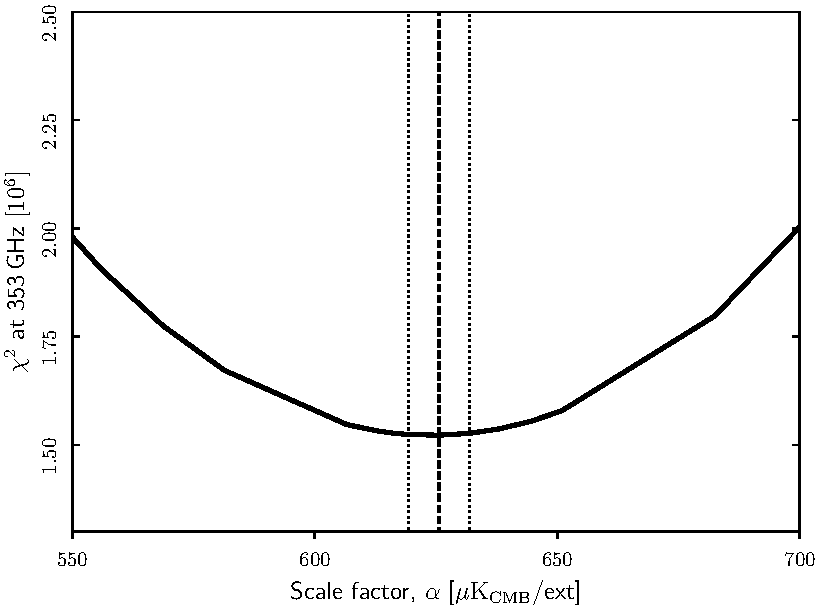
\includegraphics[width=\columnwidth]{figures/chisq_353_alpha.pdf}
  \caption{$\chi^2$ distribution for $\alpha$, the conversion factor from GAIA-based extinction to thermal dust emission at 545\,GHz, as evaluated from \Planck\ 353\,GHz data. The dashed vertical line indicates the best-fit value, and the dotted lines indicate the uncertainties. }
  \label{fig:chisq_353_alpha}
\end{figure}


\clearpage
\section{Results}
%\begin{figure}
%  \centering
%  \includegraphics[width=\columnwidth]{figures/.pdf}
%  \caption{Processing masks use in the analysis.}
%  \label{fig:masks}
%\end{figure}

\subsection{Best-fit three-component dust model}
In Figs. \ref{fig:hot_dust}, \ref{fig:cold_dust} and \ref{fig:nearby_dust}, we show typical amplitude maps for each of the three dust components in our data model.


\subsection{Correlations between our work and potential dust tracers}
\subsubsection{Hot dust}


\begin{figure}
  \centering
  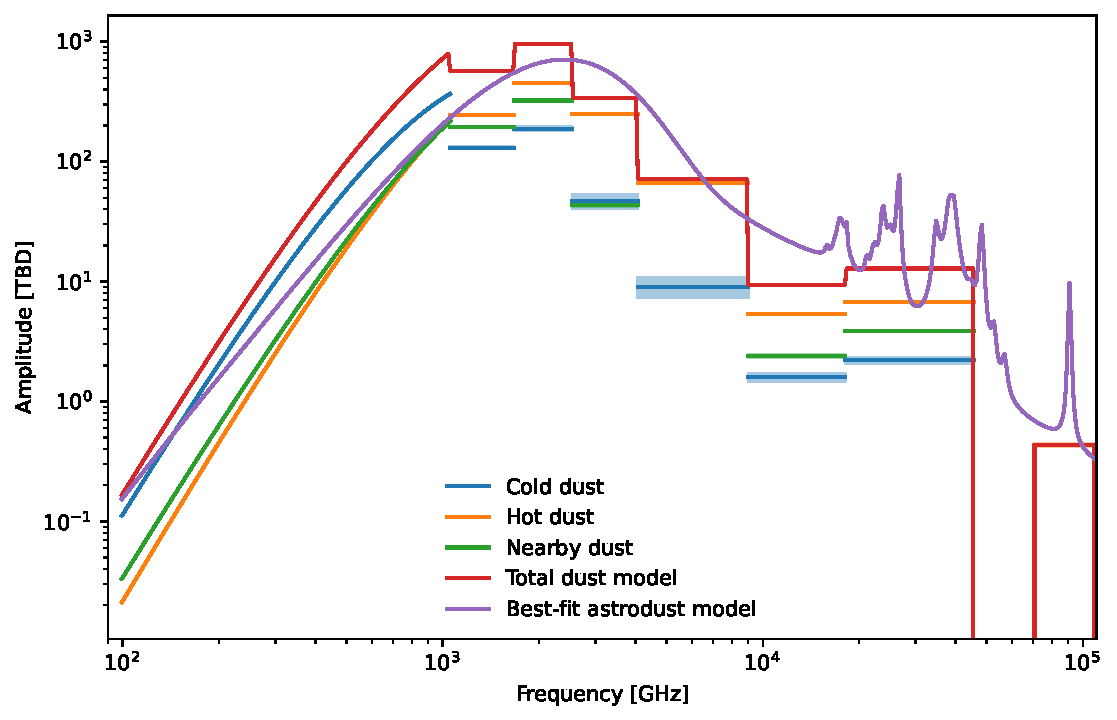
\includegraphics[width=\columnwidth]{figures/all_components_sed.pdf}
  \caption{The mean SEDs of the three dust components.}
  \label{fig:all_components_sed}
\end{figure}
\begin{figure}
  \centering
  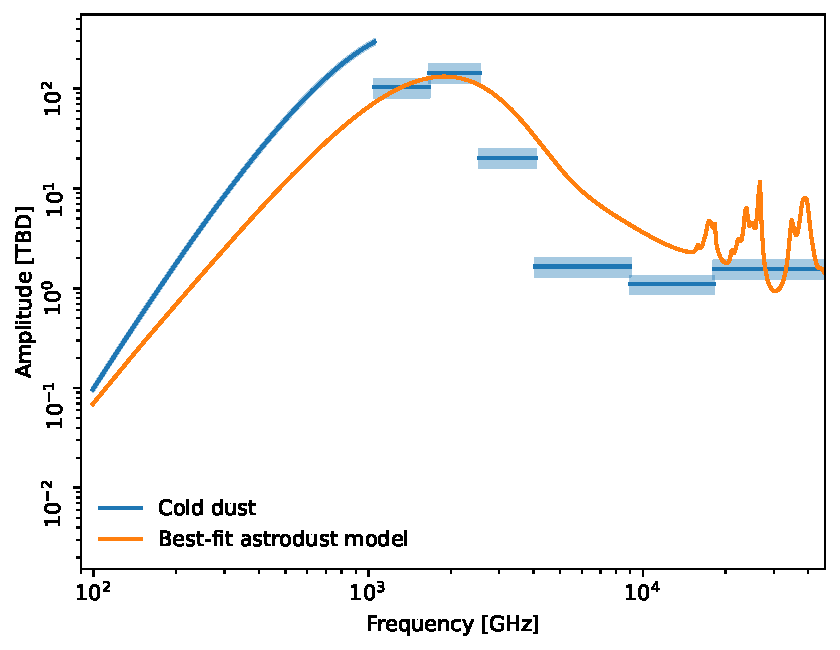
\includegraphics[width=\columnwidth]{figures/cold_dust_sed.pdf}
  \caption{The cold dust component SED.}
  \label{fig:cold_dust_sed}
\end{figure}
\begin{figure}
  \centering
  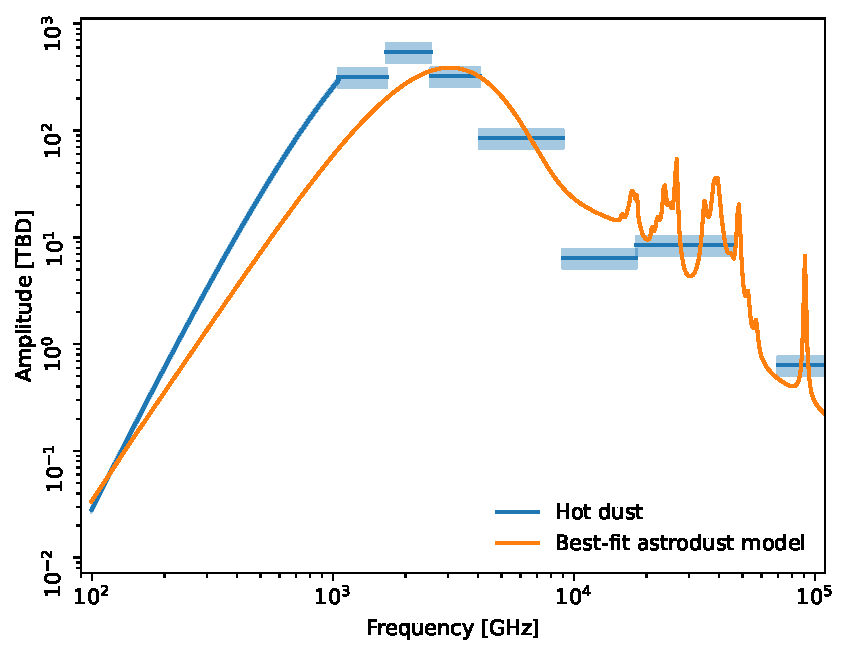
\includegraphics[width=\columnwidth]{figures/hot_dust_sed.pdf}
  \caption{The cold dust component SED.}
  \label{fig:hot_dust_sed}
\end{figure}
\begin{figure}
  \centering
  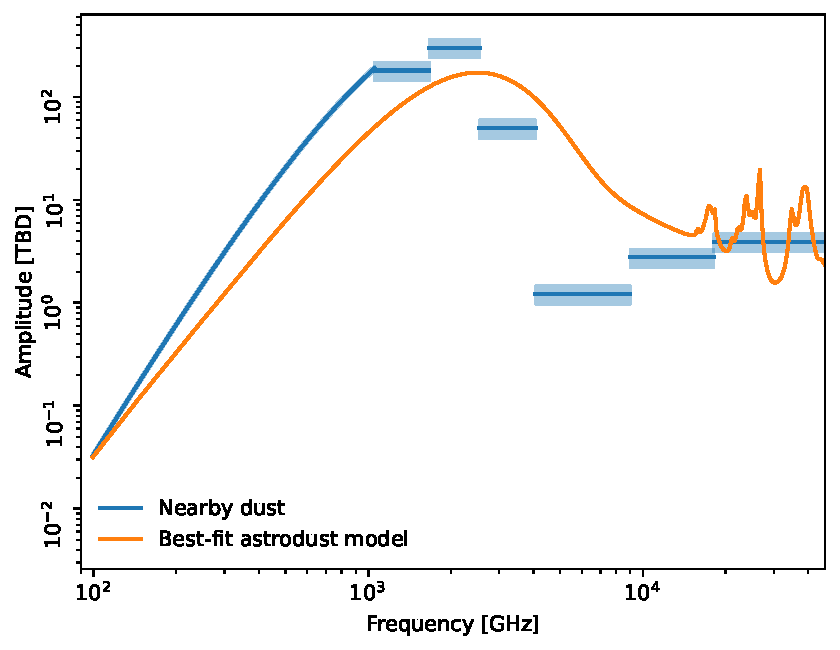
\includegraphics[width=\columnwidth]{figures/nearby_dust_sed.pdf}
  \caption{The nearby dust component SED.}
  \label{fig:nearby_dust_sed}
\end{figure}
%\begin{figure}
%  \centering
%  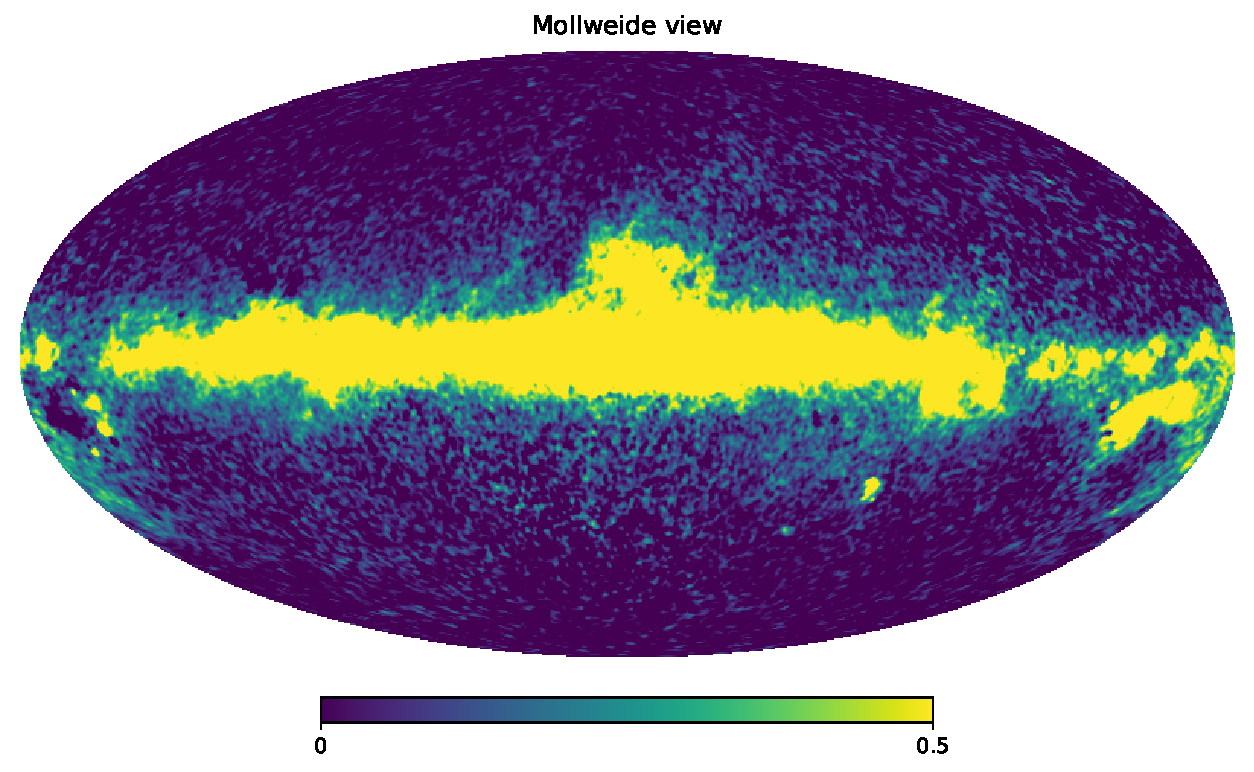
\includegraphics[width=\columnwidth]{figures/cii_DR2.pdf}
%  \caption{The DR2 CII map}
%  \label{fig:cii_DR2}
%\end{figure}
%\begin{figure}
%  \centering
%  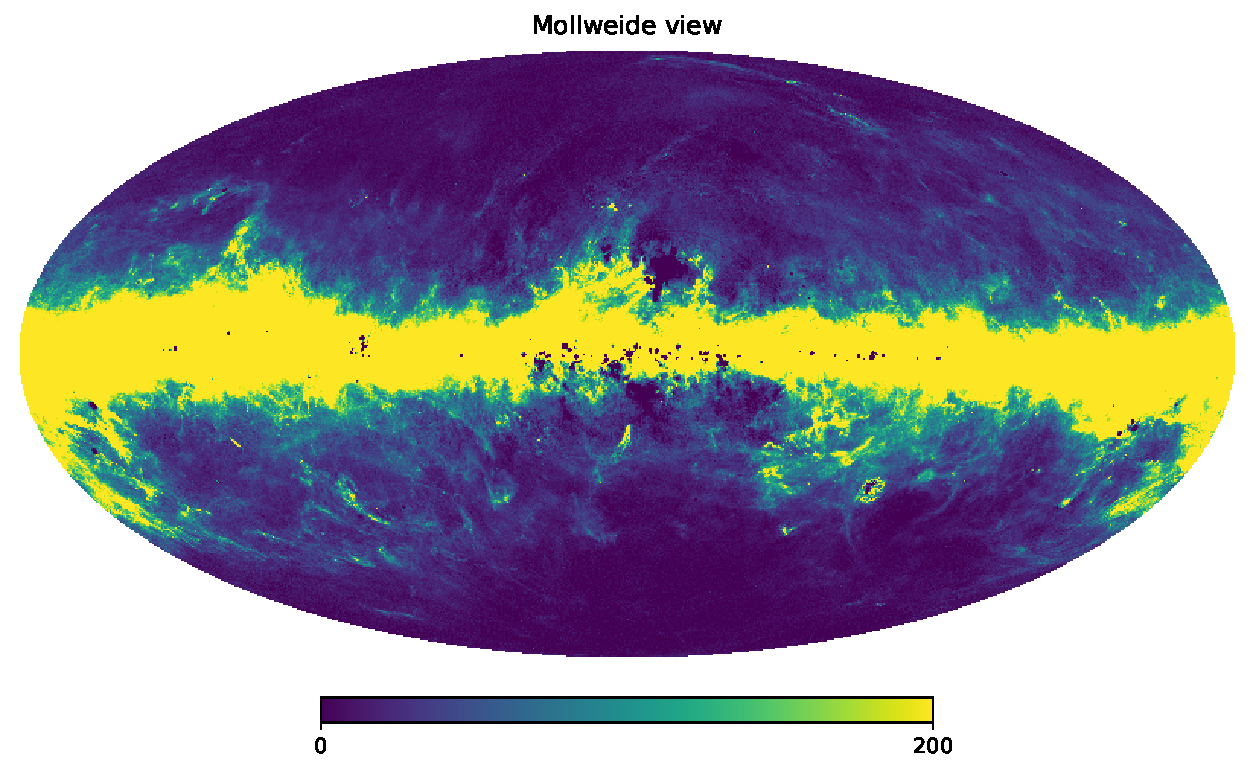
\includegraphics[width=\columnwidth]{figures/cold_dust.pdf}
%  \caption{The DR2 cold dust map}
%  \label{fig:cold_dust}
%\end{figure}
%\begin{figure}
%  \centering
%  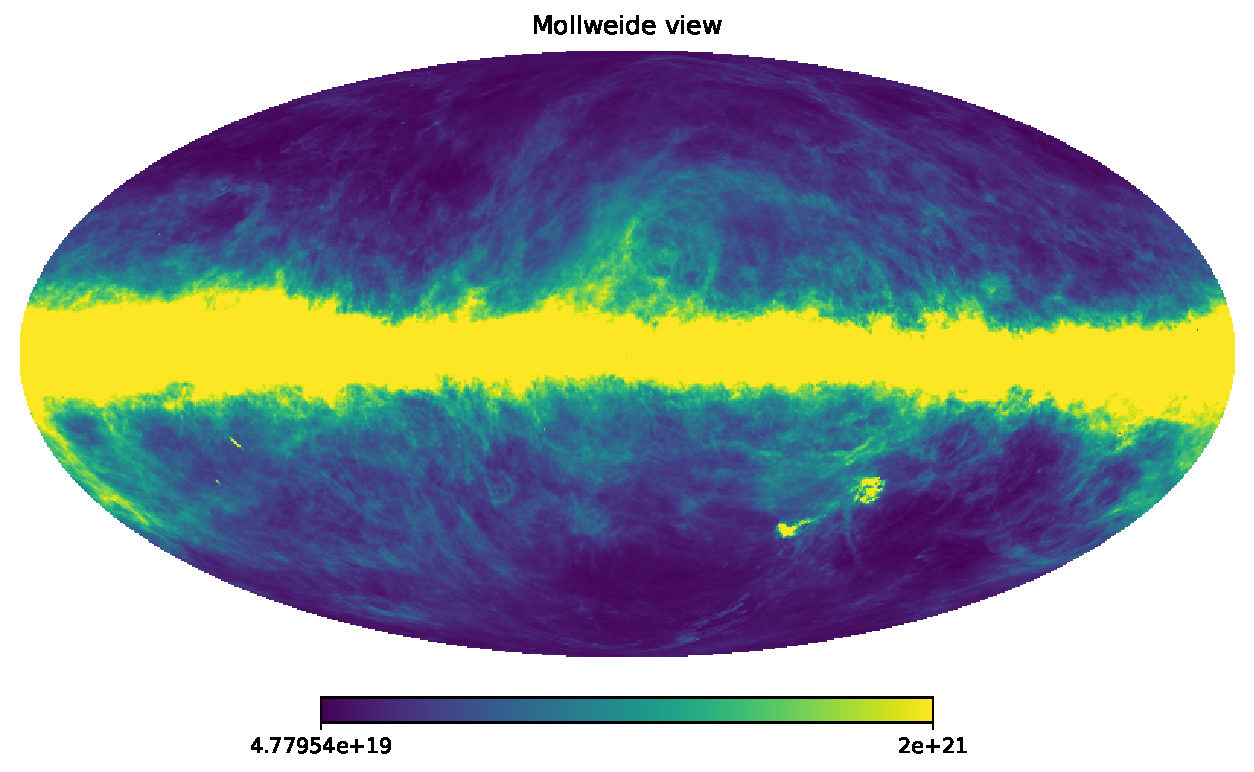
\includegraphics[width=\columnwidth]{figures/h14pi.pdf}
%  \caption{The HI4PI map}
%  \label{fig:h14pi}
%\end{figure}
%\begin{figure}
%  \centering
%  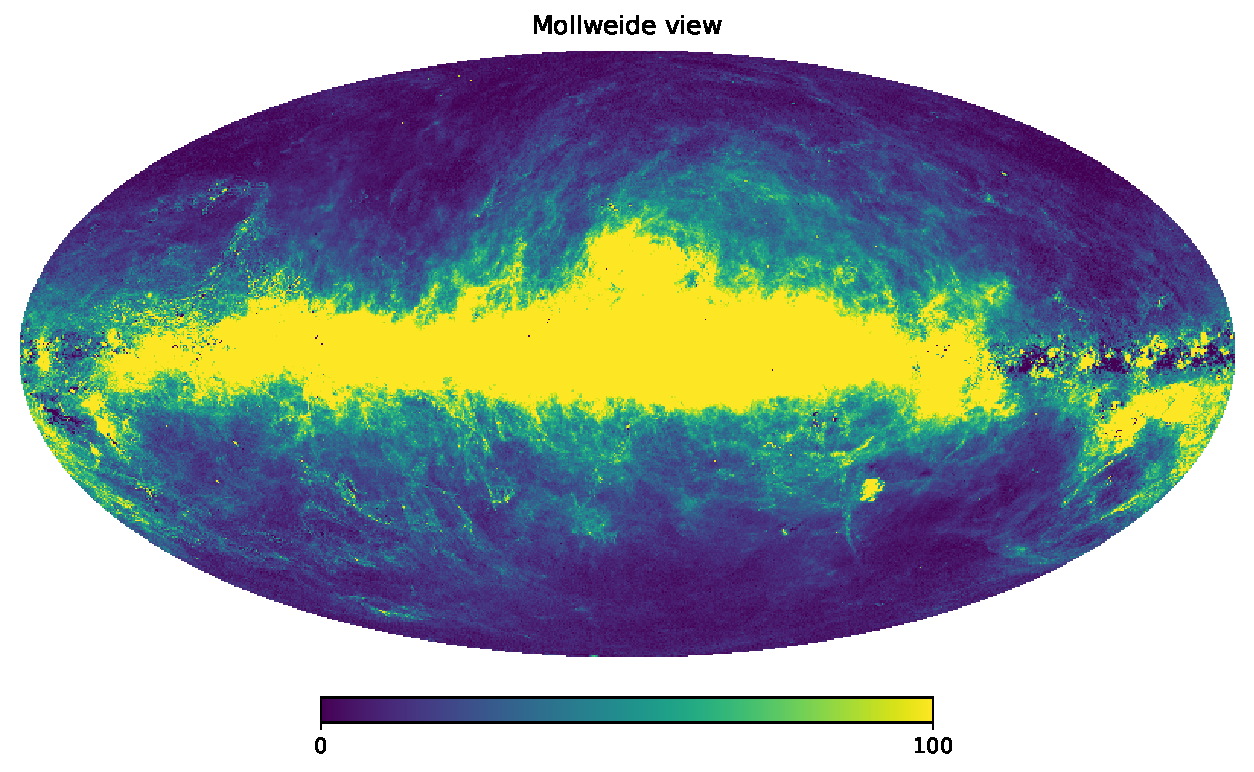
\includegraphics[width=\columnwidth]{figures/hot_dust.pdf}
%  \caption{The DR2 hot dust map}
%  \label{fig:hot_dust}
%\end{figure}
%\begin{figure}
%  \centering
%  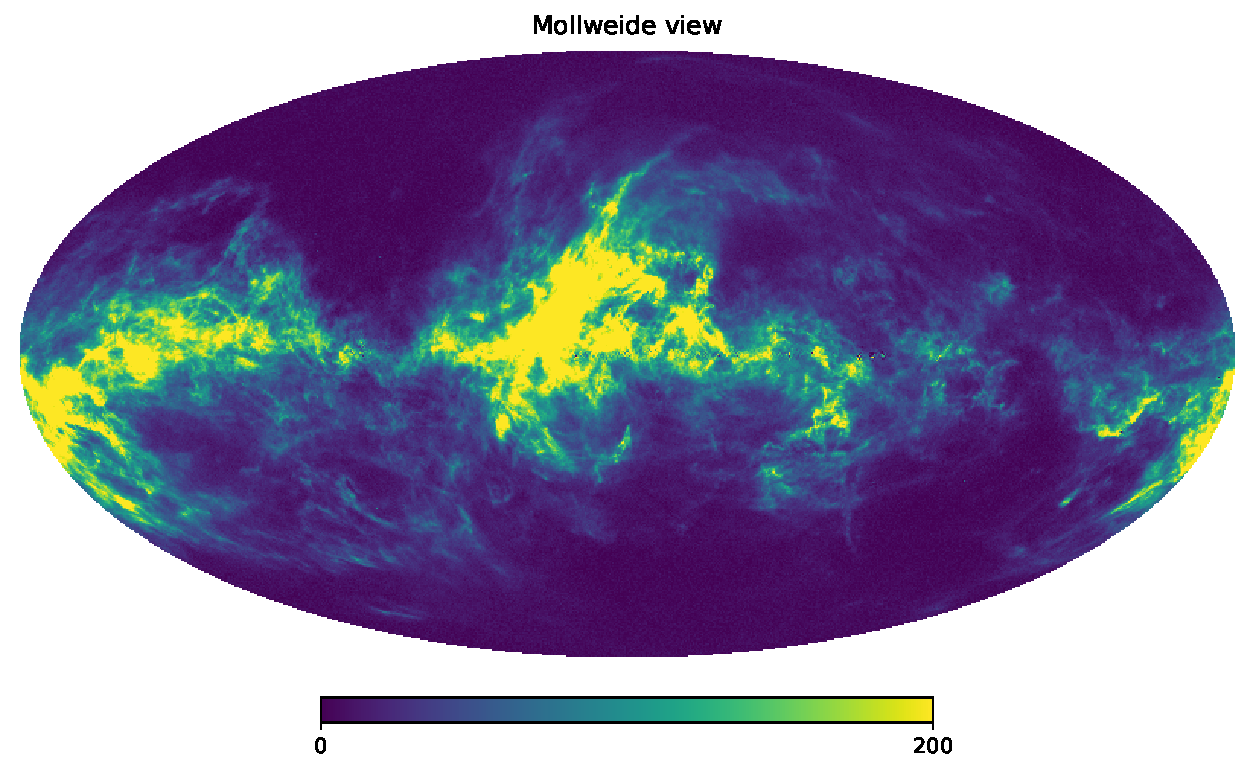
\includegraphics[width=\columnwidth]{figures/nearby_dust.pdf}
%  \caption{The DR2 nearby dust map}
%  \label{fig:nearby_dust}
%\end{figure}
%\begin{figure}
%  \centering
%  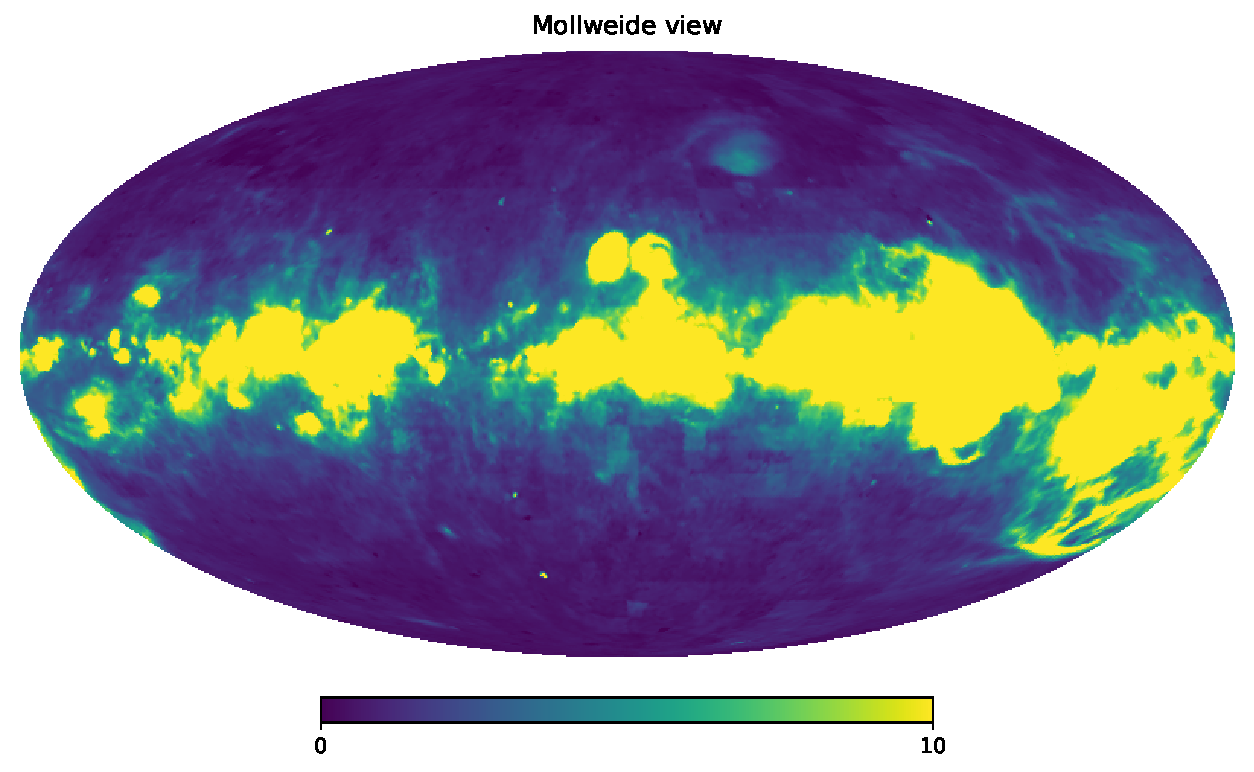
\includegraphics[width=\columnwidth]{figures/wham.pdf}
%  \caption{The WHAM map}
%  \label{fig:wham}
%\end{figure}

\begin{figure*}
  \centering
  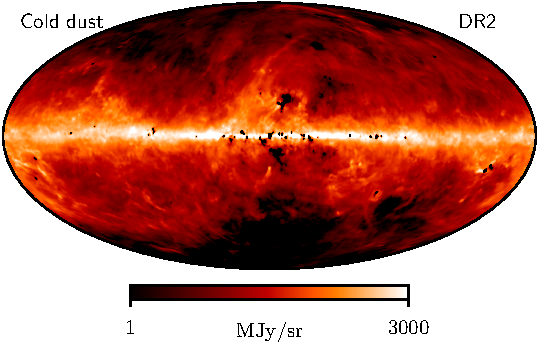
\includegraphics[width=0.49\linewidth]{figures/CGDR2_colddust_1deg_n512_v1.pdf}
  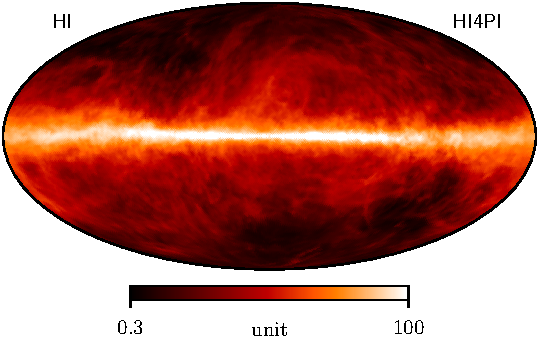
\includegraphics[width=0.49\linewidth]{figures/HI4PI_NHI_n0064_60arcmin_rescaled_TQU.pdf}\\
  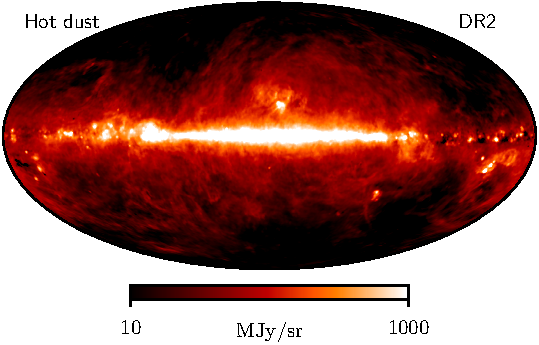
\includegraphics[width=0.49\linewidth]{figures/CGDR2_hotdust_1deg_n512_v1.pdf}
  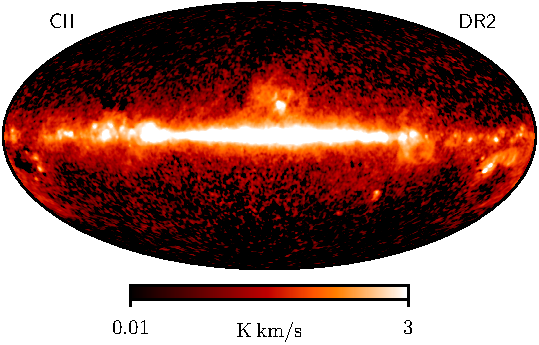
\includegraphics[width=0.49\linewidth]{figures/CGDR2_CII_1deg_n512_v1.pdf}\\
  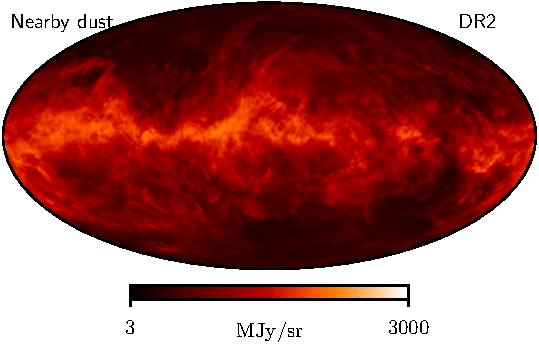
\includegraphics[width=0.49\linewidth]{figures/CGDR2_neardust_1deg_n512_v1.pdf}
  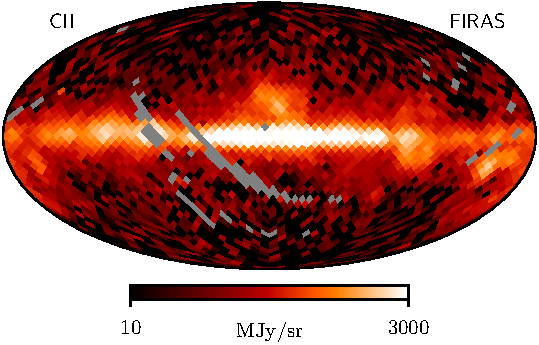
\includegraphics[width=0.49\linewidth]{figures/init_CII_firas_n16_v20.pdf}
  \caption{Comparison of \Cosmoglobe\ DR2 thermal dust maps (\emph{left column}) with respective line emission tracers (\emph{right column}). From top to bottom, the left column shows cold, hot, and nearby dust emission, respectively, while the right column shows the HI4PI surface density map, the \Cosmoglobe\ DR2 CII map derived from the DIRBE 140\,$\mu$m channel, and the FIRAS CII map.  }
  \label{fig:dustmaps}
\end{figure*}



       \begin{figure*}
         \centering
         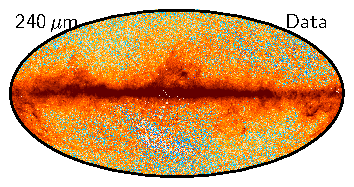
\includegraphics[width=0.19\linewidth]{figures/compfreq_mapzodi_10a_v01.pdf}
         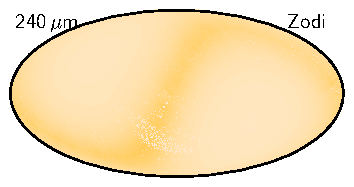
\includegraphics[width=0.19\linewidth]{figures/compfreq_zodi_10a_v01.pdf}
         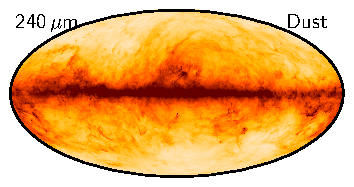
\includegraphics[width=0.19\linewidth]{figures/compfreq_dusttot_10a_v01.pdf}
         
\includegraphics[width=0.19\linewidth]{figures/compfreq_white_nobar.pdf}  
         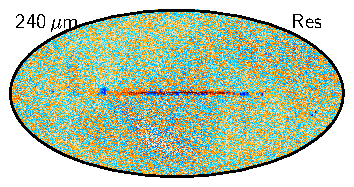
\includegraphics[width=0.19\linewidth]{figures/compfreq_todres_10a_v01.pdf}\\
         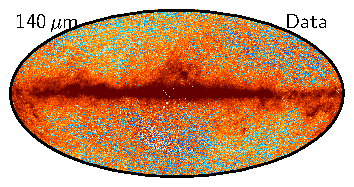
\includegraphics[width=0.19\linewidth]{figures/compfreq_mapzodi_09a_v01.pdf}
         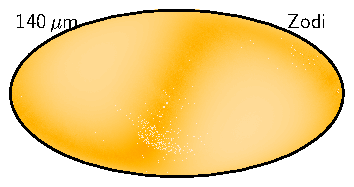
\includegraphics[width=0.19\linewidth]{figures/compfreq_zodi_09a_v01.pdf}
         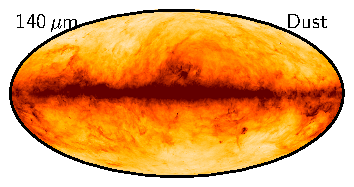
\includegraphics[width=0.19\linewidth]{figures/compfreq_dusttot_09a_v01.pdf}
         
\includegraphics[width=0.19\linewidth]{figures/compfreq_white_nobar.pdf}  
         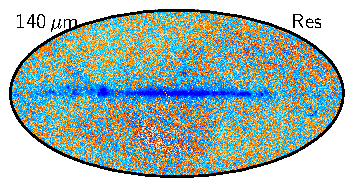
\includegraphics[width=0.19\linewidth]{figures/compfreq_todres_09a_v01.pdf}\\
         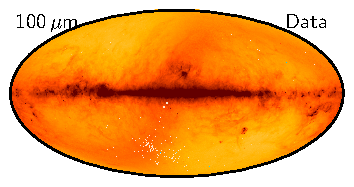
\includegraphics[width=0.19\linewidth]{figures/compfreq_mapzodi_08a_v01.pdf}
         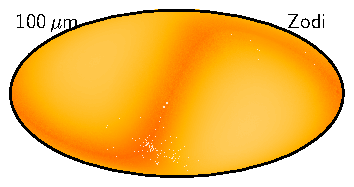
\includegraphics[width=0.19\linewidth]{figures/compfreq_zodi_08a_v01.pdf}
         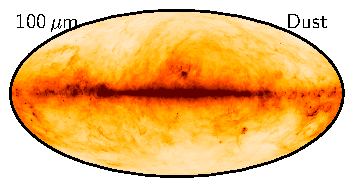
\includegraphics[width=0.19\linewidth]{figures/compfreq_dusttot_08a_v01.pdf}
         
\includegraphics[width=0.19\linewidth]{figures/compfreq_white_nobar.pdf}  
         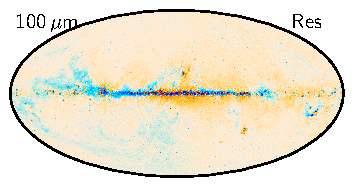
\includegraphics[width=0.19\linewidth]{figures/compfreq_todres_08a_v01.pdf}\\
         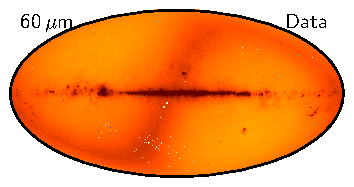
\includegraphics[width=0.19\linewidth]{figures/compfreq_mapzodi_07a_v01.pdf}
         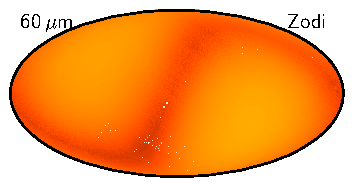
\includegraphics[width=0.19\linewidth]{figures/compfreq_zodi_07a_v01.pdf}
         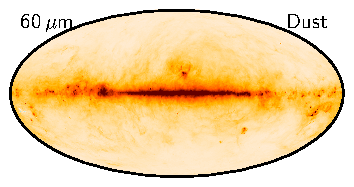
\includegraphics[width=0.19\linewidth]{figures/compfreq_dusttot_07a_v01.pdf}
         
\includegraphics[width=0.19\linewidth]{figures/compfreq_white_nobar.pdf}  
         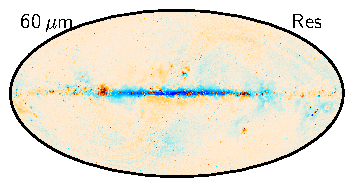
\includegraphics[width=0.19\linewidth]{figures/compfreq_todres_07a_v01.pdf}\\
         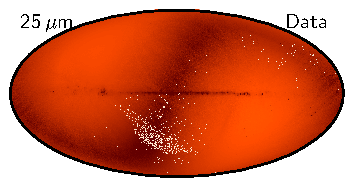
\includegraphics[width=0.19\linewidth]{figures/compfreq_mapzodi_06a_v01.pdf}
         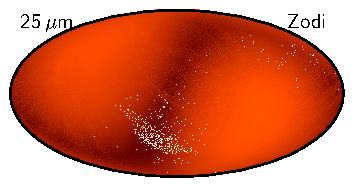
\includegraphics[width=0.19\linewidth]{figures/compfreq_zodi_06a_v01.pdf}
         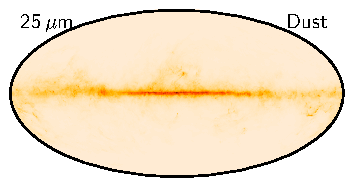
\includegraphics[width=0.19\linewidth]{figures/compfreq_dusttot_06a_v01.pdf}
         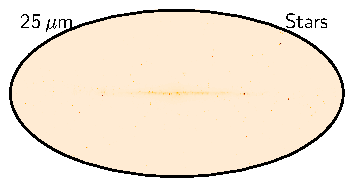
\includegraphics[width=0.19\linewidth]{figures/compfreq_stars_06a_v01.pdf}  
         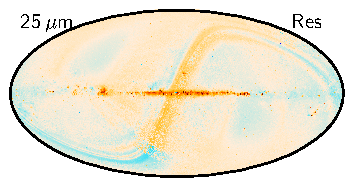
\includegraphics[width=0.19\linewidth]{figures/compfreq_todres_06a_v01.pdf}\\  
         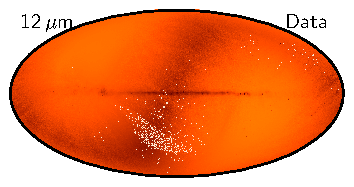
\includegraphics[width=0.19\linewidth]{figures/compfreq_mapzodi_05a_v01.pdf}
         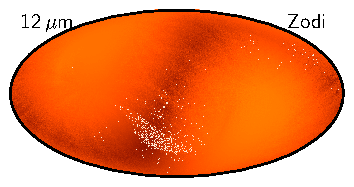
\includegraphics[width=0.19\linewidth]{figures/compfreq_zodi_05a_v01.pdf}
         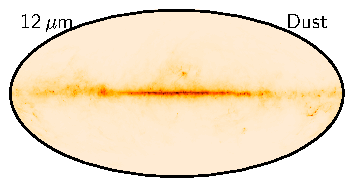
\includegraphics[width=0.19\linewidth]{figures/compfreq_dusttot_05a_v01.pdf}
         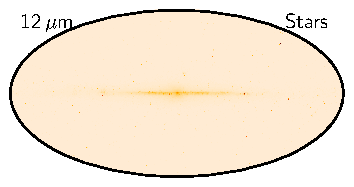
\includegraphics[width=0.19\linewidth]{figures/compfreq_stars_05a_v01.pdf}  
         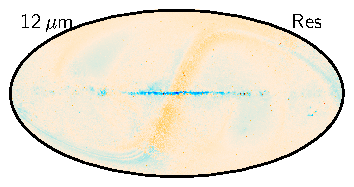
\includegraphics[width=0.19\linewidth]{figures/compfreq_todres_05a_v01.pdf}\\
         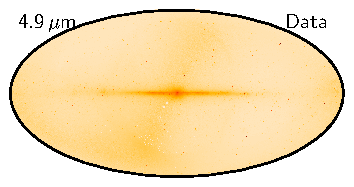
\includegraphics[width=0.19\linewidth]{figures/compfreq_mapzodi_04a_v01.pdf}
         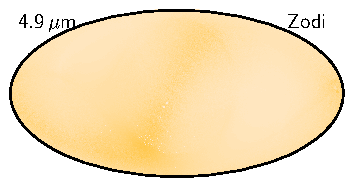
\includegraphics[width=0.19\linewidth]{figures/compfreq_zodi_04a_v01.pdf}
         \includegraphics[width=0.19\linewidth]{figures/compfreq_white_nobar.pdf}
         \includegraphics[width=0.19\linewidth]{figures/compfreq_stars_04a_v01.pdf}  
         \includegraphics[width=0.19\linewidth]{figures/compfreq_todres_04a_v01.pdf}\\  
         \includegraphics[width=0.19\linewidth]{figures/compfreq_mapzodi_03a_v01.pdf}
         \includegraphics[width=0.19\linewidth]{figures/compfreq_zodi_03a_v01.pdf}
         \includegraphics[width=0.19\linewidth]{figures/compfreq_white_nobar.pdf}
         \includegraphics[width=0.19\linewidth]{figures/compfreq_stars_03a_v01.pdf}  
         \includegraphics[width=0.19\linewidth]{figures/compfreq_todres_03a_v01.pdf}\\  
         \includegraphics[width=0.19\linewidth]{figures/compfreq_mapzodi_02a_v01.pdf}
         \includegraphics[width=0.19\linewidth]{figures/compfreq_zodi_02a_v01.pdf}
         \includegraphics[width=0.19\linewidth]{figures/compfreq_white_nobar.pdf}
         \includegraphics[width=0.19\linewidth]{figures/compfreq_stars_02a_v01.pdf}  
         \includegraphics[width=0.19\linewidth]{figures/compfreq_todres_02a_v01.pdf}\\
         \includegraphics[width=0.19\linewidth]{figures/compfreq_mapzodi_01a_v01.pdf}
         \includegraphics[width=0.19\linewidth]{figures/compfreq_zodi_01a_v01.pdf}
         \includegraphics[width=0.19\linewidth]{figures/compfreq_white_nobar.pdf}
         \includegraphics[width=0.19\linewidth]{figures/compfreq_stars_01a_v01.pdf}
         \includegraphics[width=0.19\linewidth]{figures/compfreq_todres_01a_v01.pdf}\\
         \includegraphics[width=0.50\linewidth]{figures/colourbar_MJysr.pdf}
         \caption{Comparison between the raw DIRBE data and the various fitted components for one single Gibbs sample. Columns show, from left to right, 1) the time-ordered DIRBE data co-added into pixelized maps; 2) zodiacal light emission; 3) thermal dust emission; 4) star emission; and 5) data-minus-model residual emission. Rows show individual frequency channels. Missing entries corresponds to components that are forced to zero in the model. Note that all panels are plotted with the same color scale in units of MJy/sr, and can be directly compared.}
         \label{fig:comp_vs_freq}
       \end{figure*}
       
       \begin{figure*}
       	\centering
       	\includegraphics[width=\textwidth]{figures/all_fgs.pdf}
       	\caption{Summary of all foregrounds.}
       	\label{fig:SED_overview}
       \end{figure*}



\clearpage
\section{Future directions}

\clearpage
\section{Conclusions}




\blindtext





\begin{acknowledgements}
 The current work has received funding from the European
  Union’s Horizon 2020 research and innovation programme under grant
  agreement numbers 819478 (ERC; \textsc{Cosmoglobe}) and 772253 (ERC;
  \textsc{bits2cosmology}). Some of the results in this paper have been derived using the HEALPix \citep{HEALPIX} package.
  We acknowledge the use of the Legacy Archive for Microwave Background Data
  Analysis (LAMBDA), part of the High Energy Astrophysics Science Archive Center
  (HEASARC). HEASARC/LAMBDA is a service of the Astrophysics Science Division at
  the NASA Goddard Space Flight Center.  
\end{acknowledgements}


%-------------------------------------------------------------
%                                       Table with references 
%-------------------------------------------------------------
%

\bibliographystyle{aa}
\bibliography{../../common/CG_bibliography,references,../../common/Planck_bib}
\end{document}
%%%% End of aa.dem
